\appendix
\chapter{Appendix} \label{appendix}
\section{Testing Evidence}
\begin{figure}[H]
	\centering
	
\includegraphics{images/screenshots/test-2}
	\caption{Evidence for test 2: white move, black pieces are greyed out (not clickable).}
	\label{test-2}
\end{figure}
\begin{figure}[H]
	\centering
	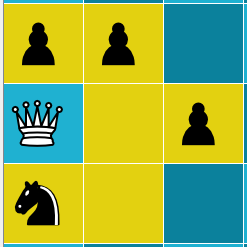
\includegraphics{images/screenshots/test-3}
	\caption{Evidence for test 3: legal moves of a queen.}
	\label{test-3}
\end{figure}
\begin{figure}[H]
	\centering
	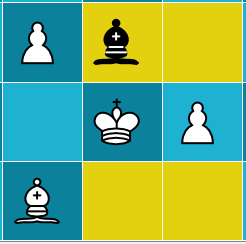
\includegraphics{images/screenshots/test-4}
	\caption{Evidence for test 4: legal moves of a king.}
	\label{test-4}
\end{figure}
\begin{figure}[H]
	\centering
	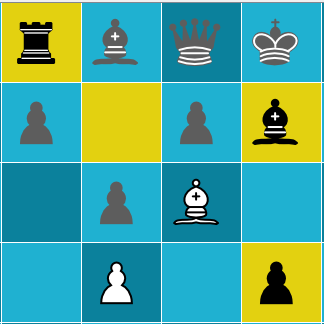
\includegraphics{images/screenshots/test-5}
	\caption{Evidence for test 5: legal moves of a bishop.}
	\label{test-5}
\end{figure}
\begin{figure}[H]
	\centering
	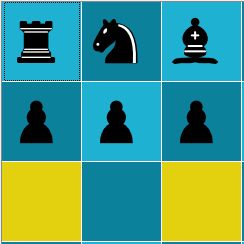
\includegraphics{images/screenshots/test-6}
	\caption{Evidence for test 6: legal moves of a knight.}
	\label{test-6}
\end{figure}
\begin{figure}[H]
	\centering
	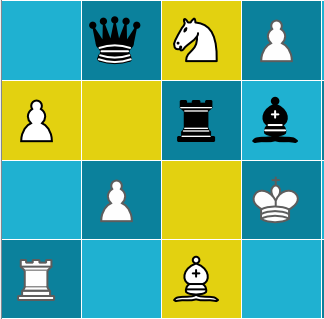
\includegraphics{images/screenshots/test-7}
	\caption{Evidence for test 7: legal moves of a rook.}
	\label{test-7}
\end{figure}
\begin{figure}[H]
	\centering
	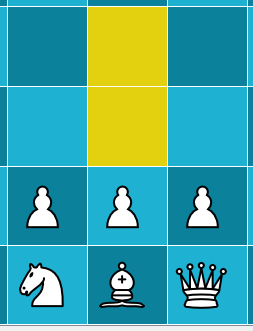
\includegraphics{images/screenshots/test-8}
	\caption{Evidence for test 8: legal moves of a pawn.}
	\label{test-8}
\end{figure}
\begin{figure}[H]
	\centering
	
\includegraphics{images/screenshots/test-9}
	\caption{Evidence for test 9: en passant move.}
	\label{test-9}
\end{figure}
\begin{figure}[H]
	\centering
	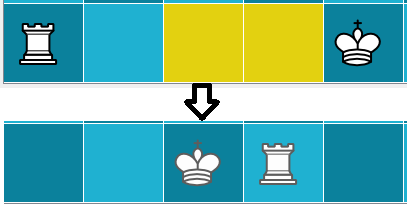
\includegraphics{images/screenshots/test-10}
	\caption{Evidence for test 10: castling move.}
	\label{test-10}
\end{figure}
\begin{figure}[H]
	\centering
	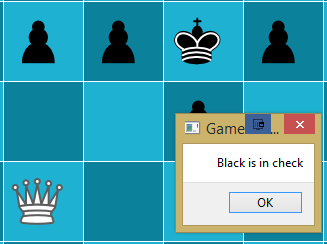
\includegraphics{images/screenshots/test-11}
	\caption{Evidence for test 11: dialog notifying user of check.}
	\label{test-11}
\end{figure}
\begin{figure}[H]
	\centering
	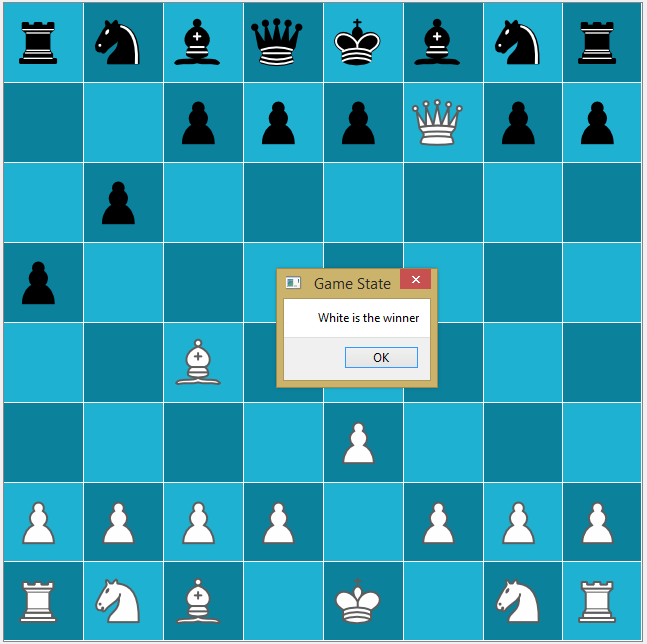
\includegraphics[width=1.0\textwidth]{images/screenshots/test-12}
	\caption{Evidence for test 12: dialog notifying user of checkmate.}
	\label{test-12}
\end{figure}
\begin{figure}[H]
	\centering
	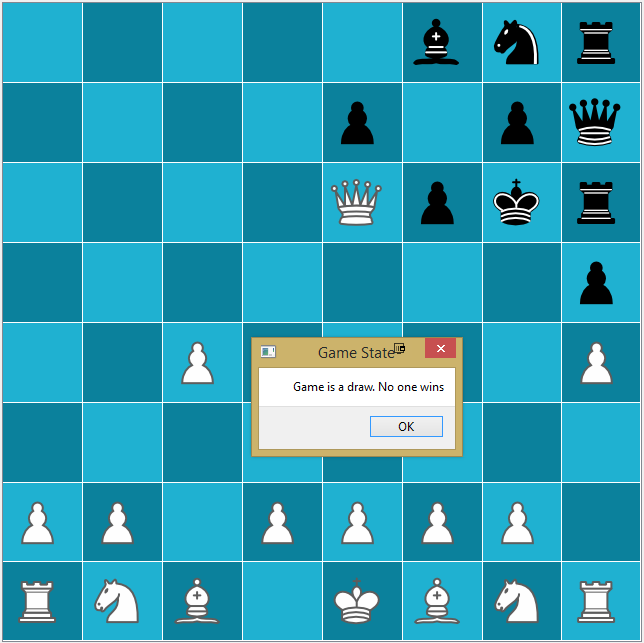
\includegraphics[width=1.0\textwidth]{images/screenshots/test-13}
	\caption{Evidence for test 13: dialog notifying user of stalemate.}
	\label{test-13}
\end{figure}
\begin{figure}[H]
	\centering
	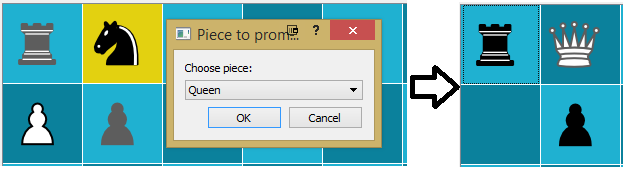
\includegraphics[width=1.0\textwidth]{images/screenshots/test-14}
	\caption{Evidence for test 14: check that promotion works.}
	\label{test-14}
\end{figure}
\begin{figure}[H]
	\centering
	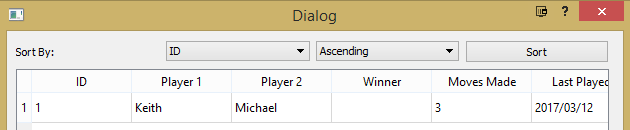
\includegraphics[width=1.0\textwidth]{images/screenshots/test-15}
	\caption{Evidence for test 15: check that game saved only when required data is filled.}
	\label{test-15}
\end{figure}
\begin{figure}[H]
	\centering
	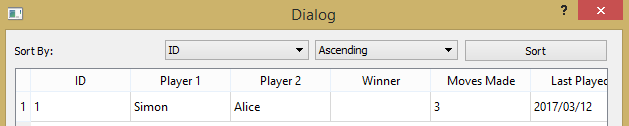
\includegraphics[width=1.0\textwidth]{images/screenshots/test-16}
	\caption{Evidence for test 16: check that game saved only when required data is filled.}
	\label{test-16}
\end{figure}
\begin{figure}[H]
	\centering
	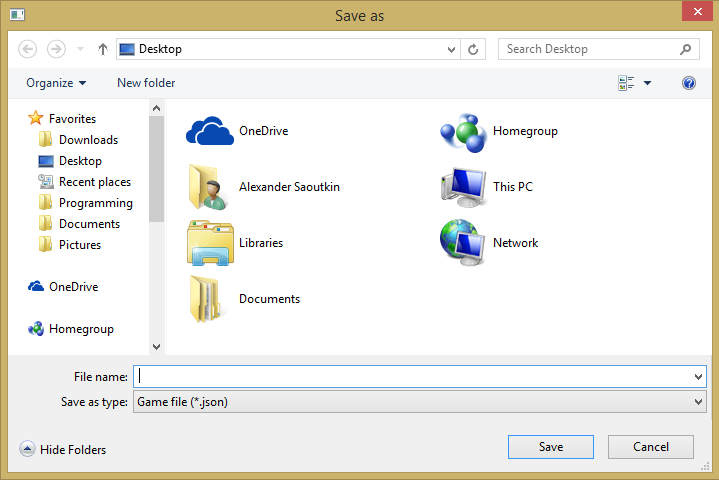
\includegraphics[width=1.0\textwidth]{images/screenshots/test-17}
	\caption{Evidence for test 17: "Save as" dialog to save game.}
	\label{test-17}
\end{figure}
\begin{figure}[H]
	\centering
	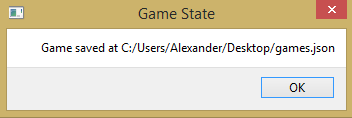
\includegraphics{images/screenshots/test-18}
	\caption{Evidence for test 18: dialog showing that game has been saved.}
	\label{test-18}
\end{figure}
\begin{figure}[H]
	\centering
	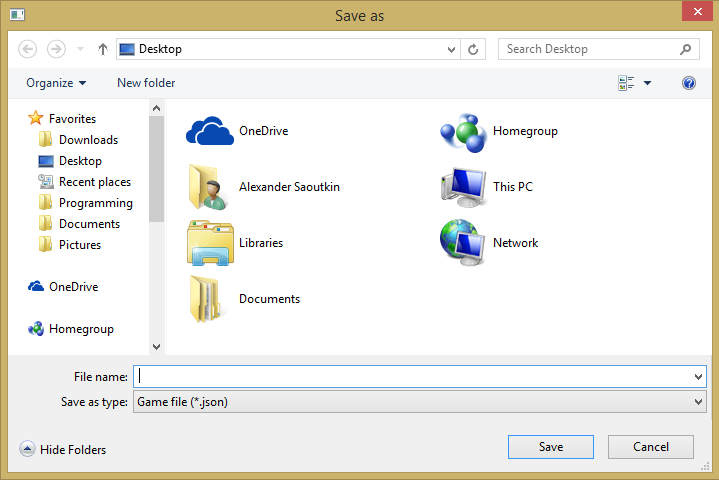
\includegraphics[width=1.0\textwidth]{images/screenshots/test-17}
	\caption{Evidence for test 19: "Save as" dialog to save game.}
	\label{test-19}
\end{figure}
\begin{figure}[H]
	\centering
	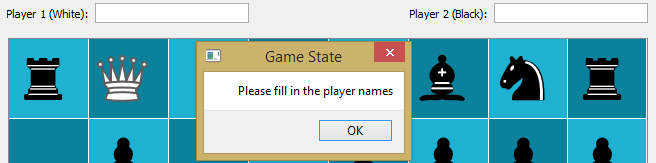
\includegraphics[width=1.0\textwidth]{images/screenshots/test-20}
	\caption{Evidence for test 20: check that game saved only when required data is filled.}
	\label{test-20}
\end{figure}
\begin{figure}[H]
	\centering
	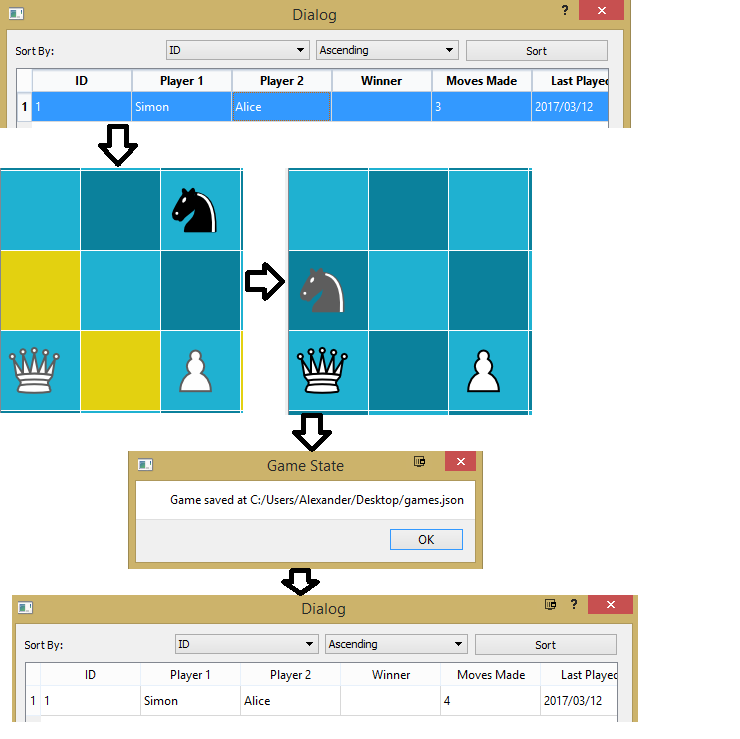
\includegraphics[width=1.0\textwidth]{images/screenshots/test-21}
	\caption{Evidence for test 21: check that game saved only when required data is filled.}
	\label{test-21}
\end{figure}
\begin{figure}[H]
	\centering
	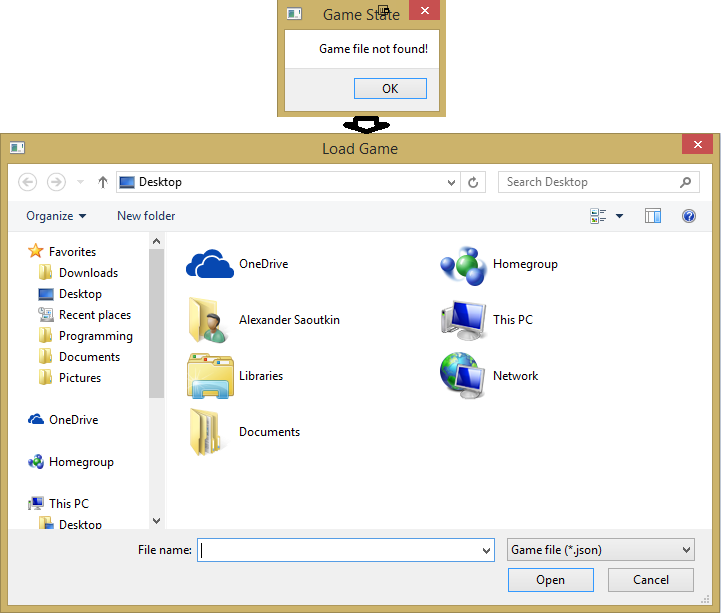
\includegraphics[width=1.0\textwidth]{images/screenshots/test-22}
	\caption{Evidence for test 22: check that game saved only when required data is filled.}
	\label{test-22}
\end{figure}
\begin{figure}[H]
	\centering
	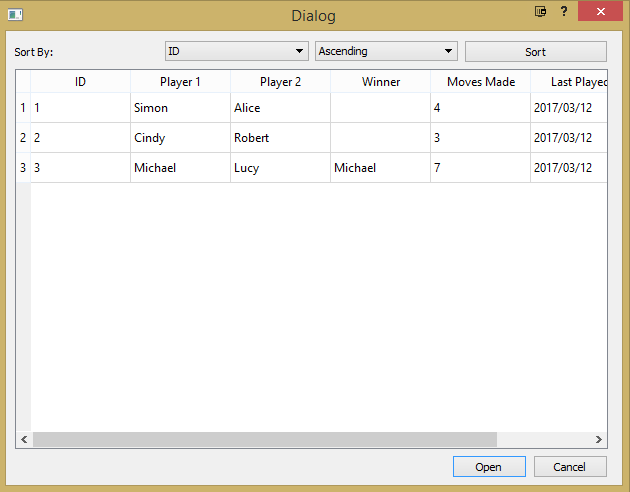
\includegraphics[width=1.0\textwidth]{images/screenshots/test-23}
	\caption{Evidence for test 23: check that game saved only when required data is filled.}
	\label{test-23}
\end{figure}
\begin{figure}[H]
	\centering
	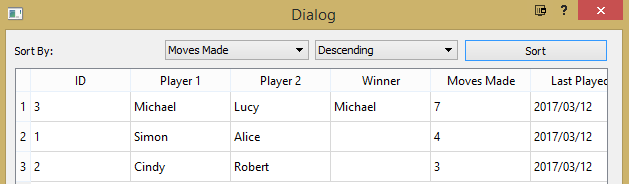
\includegraphics[width=1.0\textwidth]{images/screenshots/test-24}
	\caption{Evidence for test 24: check that game saved only when required data is filled.}
	\label{test-24}
\end{figure}
\section{Source Code}
\subsubsection{board.py}
\begin{longlisting}
	\inputminted[breaklines, linenos, breakanywhere, tabsize=4, baselinestretch=1.0, fontsize=\footnotesize]{python}{../src/board.py}
\end{longlisting}
\subsubsection{Chess.py}
\begin{longlisting}
	\inputminted[breaklines, linenos, breakanywhere, tabsize=4, baselinestretch=1.0, fontsize=\footnotesize]{python}{../src/Chess.py}
\end{longlisting}
\subsubsection{controllers.py}
\begin{longlisting}
	\inputminted[breaklines, linenos, breakanywhere, tabsize=4, baselinestretch=1.0, fontsize=\footnotesize]{python}{../src/controllers.py}
\end{longlisting}
\subsubsection{pieces.py}
\begin{longlisting}
	\inputminted[breaklines, linenos, breakanywhere, tabsize=4, baselinestretch=1.0, fontsize=\footnotesize]{python}{../src/pieces.py}
\end{longlisting}
\subsubsection{views.py}
\begin{longlisting}
	\inputminted[breaklines, linenos, breakanywhere, tabsize=4, baselinestretch=1.0, fontsize=\footnotesize]{python}{../src/views.py}
\end{longlisting}